\chapter{Automating Simple Intrusions}

.There are several way to automate an intrusion that cover
simple or sofisticated strategies,
but currently there are no complete solutions for a targeted intrusion; only
partial solutions which are handled by a human to convey a full intrusion.\nl

One of the simplest strategy to automate an intrusion is a \textbf{worm} which spreads in Internet, attacks nodes
and deploys some payload on each one,
to allow further spreading.\\
It is very simple since it does not require an attack infrastructure
\footnote{sometimes it is used to build one instead}.
Currently, worms one of the few cases that are fully automated.

\section{Worms}
A worm is a kind of malware that replicates itself onto other nodes
without human intervention.
There are several kinds of worms, depending on the way the worms spreads itself:
\begin{itemize}
   \item 
   \item Email: hide in a message or in an attachment
   \item IRC
   \item Istant Messages
   \item File sharing: hide in file that a user download
   \item Internet or network worm: attack a node through a wormable   vulnerability that affects the node
\end{itemize}
A vulnerability is \textit{wormable} if it enables a remote attack that enables remote code execution;
this results in the ability of creating a
process running on the target node.

\begin{figure}[htbp]
   \centering
   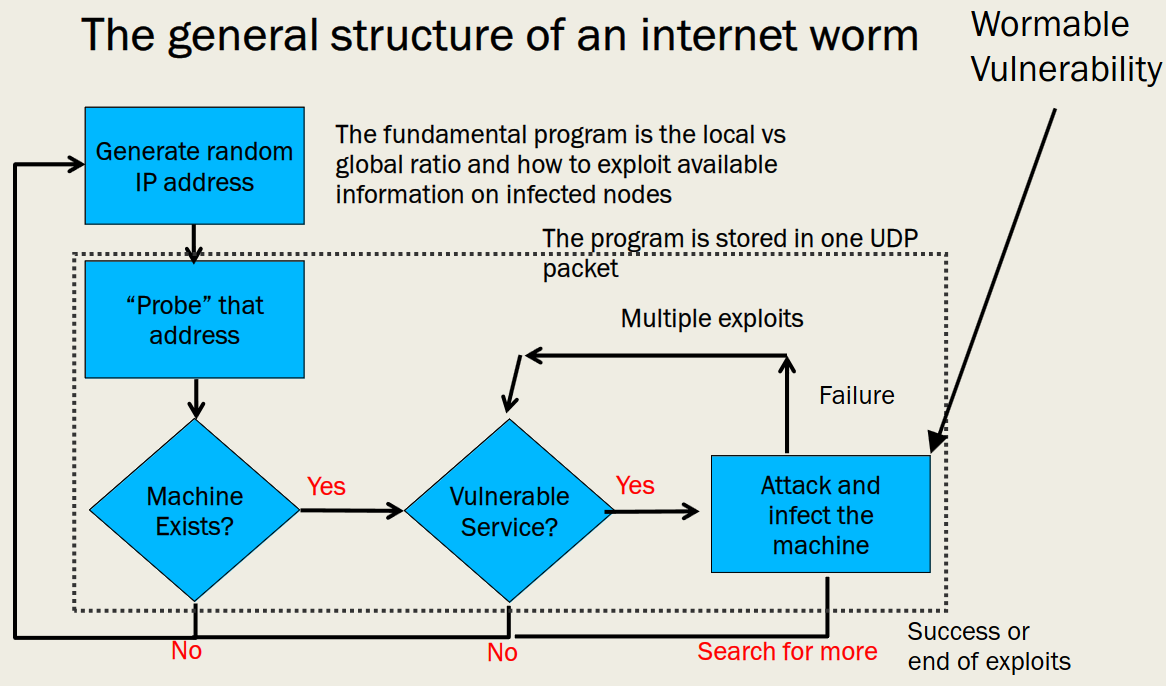
\includegraphics{images/worms_structure.png}
   \caption{Worms structure}
   \label{fig:worms_structure}
\end{figure}

\subsubsection{Obfuscation}
In several worms the code is \textbf{obfuscated} to prevent antimalware software from detecting it.\\
Each subroutine in the code can be thought of as a state machine and implemented as a
loop. 
At the start of each subroutine, the table of values is decrypted.
This table of values serves as a container for constant values used in the
subroutine, as well as the state transition table.
The malware obfuscates calls to other subroutines.
The subroutine address
is computed using hard-coded values and values from the previously
mentioned decrypted table of values. The result is placed in a register, and an
indirect call is made using the register.
A \textit{fake} \textbf{payload} is uploaded if a sandbox is detected, while the \textit{real} \textbf{payload} is a tor client.

\subsection{Domain Flux and DGA}
Most botnets use the DNS protocol to localize their C\&C servers, and some
use the \textbf{domain-flux} technique to evade blacklists.\\
Such technique implies generating a large set of pseudo-random domain names (\texttt{PDN}s) automatically.
The infected machine may contact the bot-master using a \textit{domain generation
algorithm} (\textbf{DGA}) to produce a list of candidate C\&C domains.
Then the infected machine attempts to resolve these domain names by sending
DNS queries until it obtains a successful answer from the malicious domain name reserved in advance by the bot-master.

This strategy is an \textit{effective technique} to evade detection by a monitoring system.
If one or more C\&C domain names are identified and taken down, the bots will
relocate C\&C domain name via DNS queries to the next set of automatically
generated domains.
\nl

Attackers associate multiple IP addresses with one domain name by rapidly
changing the DNS records associated with such name.
An address will be registered and then deregistered to be replaced by a new IP address every few minutes or seconds.\\
Attackers exploit a load balancing technique called \textbf{round robin DNS}, and by
setting a very short time to live (\texttt{TTL}) for each IP address. 
\note{Often, some IP
addresses will be web hosts that the attackers have compromised.}
The host acts
as proxies for the attacker's origin server.
Round robin DNS associates multiple web servers, each with its IP address, and a domain.
When the \textit{authoritative nameserver} receives a query, it hands out a
different IP address each time so that no server gets overwhelmed with traffic.\\
Attackers use this feature to obfuscate their activity.and also set a very short TTL
for these addresses as short as 60 seconds. Once the TTL expires, the address
will no longer be associated with that domain name.\\
With \textbf{double fast fluxing}, the IP address of the authoritative nameserver is also
changed out rapidly.

\subsubsection{Optimizing address generation}
Given that \textbf{density} is the probability that a random address belonging to the set corresponds to a real node,
we can define two disjoint subsets:
\begin{enumerate}
   \item \textbf{Local} (\textit{high density}), i.e. similar to the one of the infected
   node $\longrightarrow$ subnet of the infected node.
   \item \textbf{Global} (\textit{low density})
\end{enumerate}
If the ratio between \textit{local} and \textit{global} addresses is:
\begin{itemize}
   \item \textit{too low},
   the worm may be detected and removed before
   spreading
   \item \textit{too large},
   then after infecting all nodes resources are
   wasted because one node may be infected several times
\end{itemize}
\note{
   Note that even low changes in the ratio may be very critical, they create \textit{nonlinear effects}
   }

\section{A theoretical spreading model}
Let's discuss a theoretical model to study the spreading of a
worm.
The model is epidemiological, meaning that it has been defined to evaluate the overall number of people infected as a function of time:

\begin{enumerate}
   \item because of a contagious illness
   \item in a closed population
   \item fully connected population (no distancing)
\end{enumerate}

\begin{figure}[htbp]
   \centering
   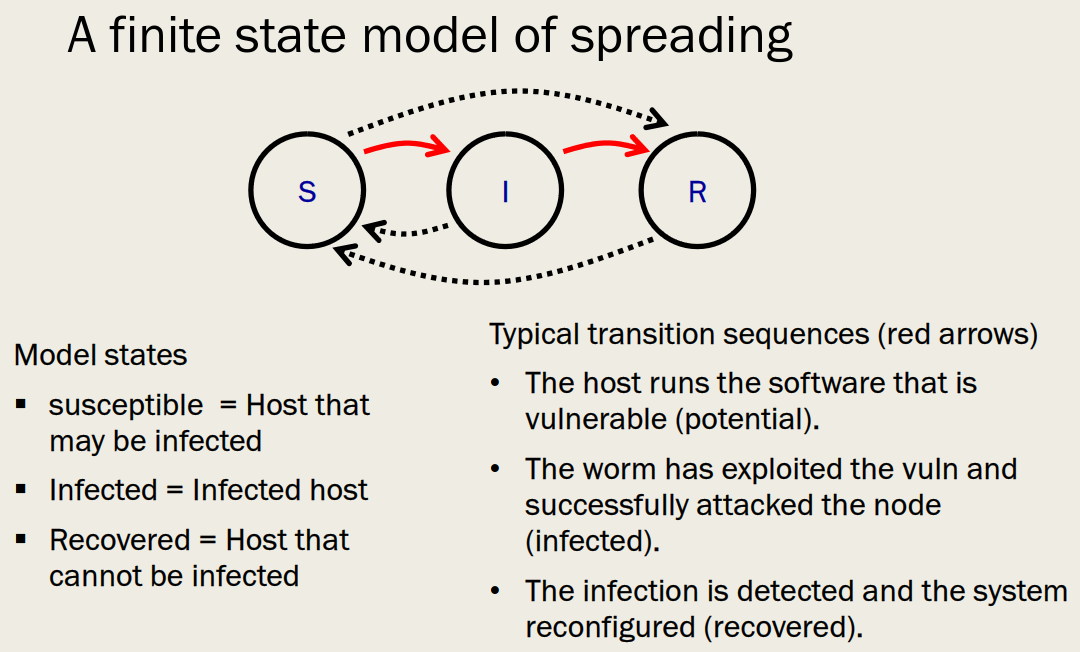
\includegraphics[width=0.45\columnwidth]{images/spreadingmodel.png}
   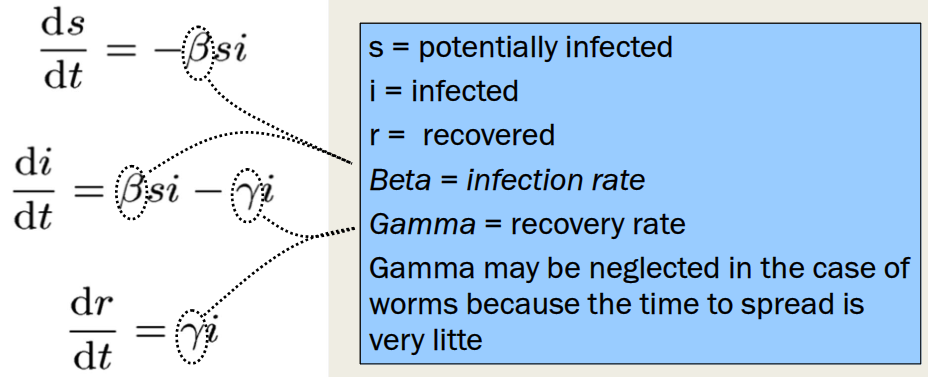
\includegraphics[width=0.45\columnwidth]{images/spreadingmodel_equations.png}
   \caption{Spreading model differential equations}
   \label{fig:spreadingmodel}
\end{figure}

\labelitemize{
   \textit{\textbf{Kermack} and \textbf{McKendrick} model}
}{
   \begin{itemize}
      \item  $\beta$ is a function of
      \begin{itemize}
         \item The function to generate the IP addresses
         \item The number of the system affected by the vulns
         \item It increase with the virulence
         \item The model assume that a node can infected any other node =
         complete connection and no defence
      \end{itemize}
      \item $\gamma$ should not be neglected anytime
      \begin{itemize}
         \item The spreading is rather slow
         \item Patching may be automated (vaccination)
         \item There are some automatic components to detect and
         remove infected nodes
      \end{itemize}
   \end{itemize}

}
